\chapter{Privasi Diferensial dan Fondasi Matematis QML}

Sebuah klinik gigi mengumpulkan catatan sepuluh ribu pasien, melatih model untuk
memprediksi siapa yang berisiko tinggi, lalu menerbitkan model itu sebagai berkas
bobot. Bulan berikutnya seorang mahasiswa mengambil satu nama dari daftar pasien yang
bocor lewat jalur lain, memasukkan rekam medis orang itu ke model, dan membaca skor
keluaran. Skornya jauh lebih tinggi daripada skor orang lain dengan rekam medis
serupa yang bukan pasien klinik itu. Mahasiswa tersebut tidak membobol basis data dan
tidak memakai kata sandi siapa pun. Ia hanya bertanya kepada model, berkali-kali, dan
model itu menjawab terlalu percaya diri untuk orang yang pernah ia lihat saat latihan.

Paralel dengan kejadian itu ada di ujung lain buku ini. Sebuah makalah melaporkan
``keunggulan kuantum'' karena sirkuitnya menyiapkan keadaan dengan $2^{50}$ amplitudo,
angka yang tidak mungkin disimpan komputer mana pun. Angka itu benar. Yang tidak
disebut makalah tersebut: amplitudo tidak bisa dibaca, dan hasil pengukuran hanya
berupa sampel.

Dua kisah itu punya cacat yang sama bentuknya: klaim berjalan lebih cepat daripada
matematika yang menopangnya. Paruh pertama bab membangun definisi yang membuat kalimat
``model ini privat'' bisa diuji, yaitu \emph{privasi diferensial}, lalu menunjukkan
mengapa definisi itu berbentuk perbandingan dua dunia dan bukan larangan mengingat.
Paruh kedua membangun fondasi untuk menilai kalimat ``model kuantum lebih unggul'':
amplitudo kompleks, gerbang uniter, aturan Born, dan biaya simulasi.

\index{privasi diferensial}
\index{keunggulan kuantum}

\kamus{privasi diferensial}{differential privacy}{janji bahwa hasil sebuah prosedur
hampir tidak berubah, dalam arti peluang, ketika satu orang masuk atau keluar dari data
latih}

\begin{untukanak}
Bayangkan sebuah toko es krim mencatat rata-rata uang belanja semua pembeli hari itu,
lalu menempelkan angka itu di pintu. Kalau Sari satu-satunya pembeli yang membeli kue
ulang tahun besar, rata-rata yang ditempel ikut naik, dan tetangga yang tahu Sari
berulang tahun bisa menebak bahwa Sari ada di daftar pembeli hari itu. Angkanya bukan
nama, tetapi angka itu tetap bercerita tentang satu orang.

Sekarang bayangkan toko yang lebih hati-hati. Sebelum menempel angka, ia menambahkan
guncangan kecil yang acak, misalnya tiga puluh sen ke atas atau ke bawah, dengan
peluang sama. Kalau Sari ikut atau tidak ikut, angka yang ditempel nyaris sama, karena
guncangan itu jauh lebih besar daripada pengaruh satu orang. Pembeli lain tetap bisa
tahu rata-rata belanja hari itu dengan cukup tepat, tetapi tidak ada lagi cara
memastikan apakah Sari ada di daftar.

Pertanyaan yang membuat penasaran: kalau guncangannya terlalu kecil, rahasianya bocor;
kalau terlalu besar, angkanya tidak berguna. Di mana batas yang jujur di antaranya, dan
bagaimana kita bisa membuktikan bahwa batas itu benar? Di bab ini kita akan tahu
mengapa janji privasi harus berbentuk perbandingan dua dunia yang nyaris identik, bukan
janji bahwa komputer akan lupa.
\end{untukanak}

\section{Apa yang bocor dari model yang dilatih pada data pribadi}
\tingkat{dasar}

Model tidak menyimpan salinan data latih. Ia menyimpan parameter, dan parameter itu
dipilih agar cocok dengan data. Justru karena pemilihan itulah data meninggalkan jejak,
dan jejak itu bisa dibaca dengan tiga cara yang berbeda tingkat kesulitannya.

Cara pertama, \emph{inferensi keanggotaan}. Penyerang punya satu rekam medis dan ingin
tahu apakah rekam itu ada di data latih. Ia tidak perlu membuka model; cukup mengirim
rekam itu dan membaca keluarannya. Model yang dilatih pada rekam tersebut biasanya
menjawab dengan keyakinan lebih tinggi, karena parameter sudah disesuaikan untuk
memasukkannya. Shokri, Stronati, Song, dan Shmatikov menunjukkan pada 2017 bahwa
perbedaan keyakinan ini cukup untuk dibedakan oleh pengklasifikasi kedua yang dilatih
pada ``model bayangan'', yaitu model tiruan yang dilatih pada data dengan dan tanpa
contoh tertentu. Serangan itu bekerja pada model yang hanya bisa ditanya, tanpa bobot
dan tanpa gradien.

Cara kedua, \emph{inferensi atribut}. Penyerang tidak menanyakan keanggotaan, melainkan
sifat yang tidak ada di data: apakah orang ini merokok, apakah ia hamil. Model yang
dilatih pada populasi tertentu bisa mengungkap korelasi yang tidak seharusnya dipakai
untuk memutuskan apa pun tentang satu orang.

Cara ketiga, \emph{rekonstruksi}: penyerang memulihkan sebagian isi data. Dinur dan
Nissim menunjukkan pada 2003 bahwa rangkaian kueri agregat berderau kecil tetap
membocorkan sebagian besar isi basis data bila kuerinya banyak dan saling bergantung.
Zhu, Liu, dan Han menunjukkan pada 2019 bahwa gradien dalam pelatihan terdistribusi
dapat dipakai untuk memulihkan gambar latih hampir persis.

Ketiga jalur itu menjelaskan mengapa kalimat ``kami hanya menerbitkan parameter, bukan
data'' tidak cukup. Yang perlu dijanjikan bukan ``tidak ada yang disalin'', melainkan
``keluaran prosedur ini hampir tidak bergantung pada satu orang''. Untuk menyatakannya
secara matematis, kita butuh dua definisi jarak: jarak antara dua himpunan data yang
berbeda pada satu orang, dan jarak antara dua sebaran keluaran.

\begin{definisi}[Pasangan data bertetangga]
Dua himpunan data $D$ dan $D'$ atas domain yang sama disebut \emph{bertetangga} bila
keduanya identik kecuali pada satu catatan: $D'$ diperoleh dari $D$ dengan menambah
atau membuang satu catatan, atau dengan mengganti satu catatan dengan catatan lain.
Himpunan semua pasangan seperti itu ditulis $\mathcal{N}$.
\end{definisi}

\index{inferensi keanggotaan}
Pilihan ``tambah atau buang'' disebut kerawanan tak terbatas, ``ganti'' disebut
kerawanan terbatas, dan keduanya memberi angka sensitivitas yang berbeda. Klaim privasi
yang tidak menyebut pilihannya belum lengkap.

\section{Definisi privasi diferensial, dan mengapa bukan rata-rata}
\tingkat{menengah}

``Hampir sama'' diukur dengan rasio peluang, bukan selisih, karena rasio tidak berubah
ketika peluangnya sangat kecil, dan justru peluang yang sangat kecil itulah yang paling
sering dipakai penyerang untuk menyimpulkan sesuatu.

\begin{definisi}[Privasi diferensial $(\varepsilon,\delta)$]
\index{privasi diferensial}
Misalkan $\varepsilon\ge 0$ dan $\delta\in[0,1]$. Prosedur acak $M$ yang memetakan
himpunan data ke ruang keluaran $\mathcal{Y}$ memenuhi privasi diferensial
$(\varepsilon,\delta)$ bila untuk setiap pasangan bertetangga $(D,D')\in\mathcal{N}$ dan
setiap himpunan terukur $S\subseteq\mathcal{Y}$ berlaku
\begin{equation}
P\bigl[M(D)\in S\bigr] \;\le\; e^{\varepsilon}\,P\bigl[M(D')\in S\bigr] + \delta .
\end{equation}
Bila $\delta=0$, prosedur itu memenuhi privasi diferensial murni $\varepsilon$.
\end{definisi}

\begin{figure}[htbp]
\centering
\begin{tikzpicture}
\begin{axis}[width=6.2cm,height=4.1cm,xmin=-2.6,xmax=3.6,ymin=0,ymax=4.6,
  domain=-2.6:3.6,samples=200,axis lines=left,
  xtick={-2,-1,0,1,2,3},ytick={0,2,4},
  tick label style={font=\scriptsize},label style={font=\scriptsize},
  title={$\varepsilon=8$},title style={font=\scriptsize},
  xlabel={keluaran},ylabel={kerapatan},
  legend style={font=\scriptsize,draw=none,at={(0.03,0.97)},anchor=north west},
  legend cell align=left]
  \addplot[thick,accent,fill=accent!12] {4*exp(-8*abs(x))} \closedcycle;
  \addlegendentry{data $D$}
  \addplot[thick,layerteal,densely dashed] {4*exp(-8*abs(x-1))};
  \addlegendentry{data $D'$}
\end{axis}
\end{tikzpicture}
\hfill
\begin{tikzpicture}
\begin{axis}[width=6.2cm,height=4.1cm,xmin=-2.6,xmax=3.6,ymin=0,ymax=0.142,
  domain=-2.6:3.6,samples=200,axis lines=left,
  xtick={-2,-1,0,1,2,3},ytick={0,0.05,0.1},yticklabels={$0$,$0{,}05$,$0{,}1$},
  tick label style={font=\scriptsize},label style={font=\scriptsize},
  title={$\varepsilon=0{,}25$},title style={font=\scriptsize},
  xlabel={keluaran},
  legend style={font=\scriptsize,draw=none,at={(0.03,0.97)},anchor=north west},
  legend cell align=left]
  \addplot[thick,accent,fill=accent!12] {0.125*exp(-0.25*abs(x))} \closedcycle;
  \addlegendentry{data $D$}
  \addplot[thick,layerteal,densely dashed] {0.125*exp(-0.25*abs(x-1))};
  \addlegendentry{data $D'$}
\end{axis}
\end{tikzpicture}
\caption{Sebaran keluaran mekanisme Laplace pada sensitivitas $1$ untuk dua basis
data bertetangga yang berbeda satu catatan, dengan skala tegak berbeda di kedua
panel. Pada $\varepsilon=8$ kedua kurva terpisah jauh, sehingga satu keluaran
sudah cukup untuk menebak data mana yang dipakai. Pada $\varepsilon=0{,}25$
keduanya hampir berimpit: rasio ordinatnya di setiap titik paling besar
$e^{0{,}25}\approx1{,}284$, jadi satu keluaran hampir tidak memihak salah satu
data.}
\label{fig:dua-sebaran}
\end{figure}

Pembaca baru biasanya bertanya dua hal: mengapa perbandingan peluang, bukan rata-rata,
dan mengapa ada $\delta$ sama sekali kalau $\varepsilon$ sudah mengukur kebocoran.

Jawaban pertanyaan pertama adalah inti paruh pertama bab. Perhatikan urutan kuantornya:
\emph{untuk setiap} $S$, \emph{untuk setiap} pasangan bertetangga. Janji itu harus
berlaku bagi uji $S$ mana pun, termasuk uji yang dipilih penyerang setelah ia melihat
mekanismenya. Definisi yang berbentuk rata-rata menempatkan kuantor di dalam: ``ada
harapan yang kecil''. Dua bentuk itu tidak setara; Gambar~\ref{fig:dua-sebaran}
menunjukkan bedanya pada dua nilai $\varepsilon$.

\begin{proposisi}
Misalkan $M$ memenuhi privasi diferensial $(\varepsilon,0)$. Maka untuk setiap algoritme
penyerang $A$ yang keluarannya hanya $0$ atau $1$, dan setiap pasangan bertetangga
$(D,D')$,
\begin{equation}
P\bigl[A\bigl(M(D)\bigr)=1\bigr] \;\le\; e^{\varepsilon}\,
P\bigl[A\bigl(M(D')\bigr)=1\bigr] .
\end{equation}
\end{proposisi}

\begin{proof}
Himpunan $\{y : A(y)=1\}$ terukur, jadi ia boleh dipakai sebagai $S$ pada definisi.
Substitusi langsung memberi hasilnya.
\end{proof}

Proposisi itu terlihat sepele, dan gunanya justru menutup pintu yang sering dipakai
untuk membela mekanisme lemah. Kalau janji hanya berlaku untuk \emph{rata-rata}
keluaran, penyerang bisa merata-ratakan hasil banyak pengulangan sehingga komponen acak
saling menghapus dan yang tinggal adalah sinyal tentang satu orang. Dengan janji
per-kejadian, setiap pengulangan membayar anggaran privasi sendiri.

\begin{bacakeras}
Baca bergantian, dua suara. Suara pertama bertanya, suara kedua menjawab.

``Kalau satu orang keluar dari daftar, apakah jawabanmu berubah?''\\
``Sedikit.''\\
``Berapa sedikit?''\\
``Cukup sedikit sehingga tidak ada yang bisa memastikan.''

Ulangi percakapan itu tiga kali, makin cepat, sampai terasa seperti hafalan. Lalu
suara pertama bertanya lagi, lebih pelan:

``Kalau pertanyaan itu kuulang seratus kali, apakah seratus kali sedikit masih
sedikit?''

Diam satu tarikan napas. Jawab berdua: sedikit yang diulang seratus kali bukan sedikit
lagi. Lalu ucapkan bersama, satu kali: satu orang tidak boleh mengubah kesimpulan.
Ulangi baris itu sekali lagi, lebih lambat, lalu sekali lagi sambil menunjuk satu kursi
kosong di ruangan.
\end{bacakeras}

\begin{contoh}[Jawaban acak]
\index{jawaban acak}
Seorang responden ditanya apakah ia pernah memakai obat terlarang. Prosedurnya: lempar
koin; bila muncul sisi A, jawab jujur; bila muncul sisi B, lempar lagi dan jawab ``ya''
bila gambar, ``tidak'' bila angka. Peluang menjawab ``ya'' bila ia benar-benar memakai
adalah $1/2+1/2\cdot 1/2=3/4$, dan bila tidak memakai adalah $1/2\cdot 1/2=1/4$.
Rasio keduanya $3$, sehingga $\varepsilon=\ln 3=1{,}0986$. Tidak ada jawaban yang
membuktikan apa pun tentang satu orang, dan itulah yang dijanjikan definisi.
\end{contoh}

\begin{tangan}
Bahan: satu koin per orang, kertas, pensil. Sepuluh teman masing-masing menulis satu
rahasia ya/tidak pada sobekan kertas dan melipatnya.

Aturannya satu. Lempar koin: gambar, jawab jujur; angka, lempar lagi, gambar berarti
``ya'' dan angka berarti ``tidak''. Setiap orang hanya menyebut satu kata, dan pencatat
hanya menulis dua kelompok turus.

Sekarang minta satu orang mengganti rahasianya, lalu ulangi seluruh putaran. Lihat
turusnya: bergeser paling banyak satu, dan tidak ada yang bisa menunjuk siapa pun.
Kesimpulan tentang kelompok bertahan. Kesimpulan tentang satu orang tidak pernah muncul.
\end{tangan}

Sekarang $\delta$, yaitu peluang kegagalan: dengan peluang paling besar $\delta$, janji
rasio tadi boleh dilanggar sepenuhnya. Karena itu $\delta$ bukan toleransi yang bisa
dipilih sesuka hati. Bila $\delta$ sebanding dengan $1/n$ untuk $n$ catatan, penyerang
bisa menargetkan satu orang dan membiarkan sisanya sebagai samaran; karena itu $\delta$
harus jauh lebih kecil daripada $1/n$. Angka $\varepsilon$ juga bukan peluang:
$\varepsilon=1$ berarti rasio peluang paling besar $e\approx 2{,}718$, sedangkan
$\varepsilon=8$ berarti rasio sampai $2\,981$.

\section{Sensitivitas global dan mekanisme Laplace}
\tingkat{menengah}

Satu-satunya hal yang menghalangi kita menambah derau secara sembarang adalah
pertanyaan: seberapa besar satu catatan bisa menggeser jawaban?

\begin{definisi}[Sensitivitas global]
\index{sensitivitas global}
Untuk $f$ yang memetakan himpunan data ke $\mathbb{R}^d$, sensitivitas globalnya adalah
\begin{equation}
\Delta f \;=\; \sup_{D\sim D'} \bigl\| f(D)-f(D') \bigr\|_{1},
\end{equation}
dengan supremum diambil atas semua pasangan bertetangga.
\end{definisi}

Kueri hitung, $f(D)=|D|$, punya $\Delta f=1$. Kueri jumlah atas nilai dalam $[0,R]$
punya $\Delta f=R$. Kueri rata-rata atas $n$ catatan punya $\Delta f=R/n$, karena satu
orang hanya menggeser rata-rata sebesar $R/n$; di sinilah terlihat bahwa rata-rata lebih
aman daripada jumlah, tetapi hanya selama $n$ diketahui dan tetap. Sensitivitas juga
bergantung pada pilihan ketetanggaan: bila $D'$ boleh mengganti, kueri hitung punya
$\Delta f=2$.

\begin{teorema}[Mekanisme Laplace]
\index{mekanisme Laplace}
Misalkan $f$ punya sensitivitas global $\Delta f$, dan $Y$ berdistribusi Laplace dengan
skala $b=\Delta f/\varepsilon$, yaitu dengan kepadatan $p_b(y)=\frac{1}{2b}e^{-|y|/b}$.
Maka $M(D)=f(D)+Y$ memenuhi privasi diferensial $(\varepsilon,0)$.
\end{teorema}

\begin{proof}
Ambil $S\subseteq\mathbb{R}$ terukur dan $D\sim D'$. Cukup ditunjukkan bahwa untuk
setiap $y$,
\begin{equation}
\frac{p_b\bigl(y-f(D)\bigr)}{p_b\bigl(y-f(D')\bigr)} \;\le\; e^{\varepsilon}.
\end{equation}
Dengan $a=f(D)$ dan $a'=f(D')$, ruas kiri adalah $\exp\bigl((|y-a'|-|y-a|)/b\bigr)$.
Pertidaksamaan segitiga memberi $|y-a'|-|y-a|\le|a-a'|$, sehingga ruas kiri paling
besar $\exp(|a-a'|/b)\le\exp(\Delta f/b)=e^{\varepsilon}$, karena $\Delta f$ adalah
supremum. Jadi $p_b(y-a)\le e^{\varepsilon}p_b(y-a')$ untuk setiap $y$; integrasi kedua
ruas atas $S$ memberi $P[M(D)\in S]\le e^{\varepsilon}P[M(D')\in S]$, dan karena tidak
ada suku sisa, $\delta=0$.
\end{proof}

Angka contohnya begini. Untuk kueri hitung dengan $\varepsilon=0{,}5$, skala
$b=1/0{,}5=2$; peluang derau melebihi $5$ dalam nilai mutlak adalah $e^{-5/2}=0{,}0821$,
jadi sekitar satu dari dua belas jawaban meleset lebih dari lima orang. Sebaliknya
dengan peluang $0{,}95$ galatnya tidak melebihi $b\ln 20=2\times 2{,}9957=5{,}991$. Di
sini terlihat bentuk trade-off yang berulang sepanjang bab: mengecilkan $\varepsilon$
memperbesar $b$, dan memperbesar $b$ memperburuk ketelitian secara linear.

\begin{resep}
\begin{enumerate}
  \item Tetapkan $f$ dan potong setiap nilai ke rentang $[0,R]$ sebelum apa pun dihitung.
  \item Hitung $\Delta f$ dari kasus terburuk satu catatan pada data yang sudah terpotong.
  \item Pilih $\varepsilon>0$, hitung $b=\Delta f/\varepsilon$, tambahkan derau Laplace
        berskala $b$ pada jawaban.
  \item Catat $\varepsilon$ pada buku anggaran; sisa anggaran adalah yang belum dipakai.
\end{enumerate}
Peringatan urutan: memotong setelah derau ditambahkan mengubah sebaran keluaran dan
membatalkan jaminan, karena $\Delta f$ dihitung dari data yang belum terpotong.
\end{resep}

\kamus{sensitivitas global}{global sensitivity}{seberapa jauh satu orang bisa menggeser
jawaban sebuah kueri pada kasus terburuk; inilah yang menentukan besar derau yang
dibutuhkan}

Kadang derau Laplace tidak cocok, misalnya karena keluarannya berdimensi tinggi. Di situ
dipakai derau Gauss: untuk $f$ dengan sensitivitas $\ell_2$ sebesar $\Delta_2 f$,
mekanisme $M(D)=f(D)+N(0,\sigma^{2}\Delta_2 f^{2}I)$ memenuhi $(\varepsilon,\delta)$
bila $\sigma\ge\sqrt{2\ln(1{,}25/\delta)}/\varepsilon$. Buktinya dilewati di sini; ia
membandingkan dua normal yang digeser dengan pertidaksamaan konsentrasi, dan lengkapnya
ada pada Dwork dan Roth (2014), lampiran A. Syarat itu cukup, bukan perlu: untuk $\sigma$ kecil ia jauh lebih longgar
daripada batas sebenarnya, dan batas ketatnya diberikan mekanisme Gauss analitik Balle
dan Wang (2018).

\section{Komposisi: anggaran privasi dan mengapa ia habis}
\tingkat{lanjut}

Satu mekanisme jarang dipakai sekali. Model dilatih dengan ratusan langkah, masing-masing
membocorkan sedikit, dan yang dibutuhkan adalah totalnya.

\begin{teorema}[Komposisi dasar]
\index{komposisi}
Misalkan $M_1,\dots,M_T$ dipilih secara adaptif, yaitu $M_t$ boleh bergantung pada
keluaran $M_1,\dots,M_{t-1}$, dan setiap $M_t$ memenuhi $(\varepsilon_t,\delta_t)$
untuk semua masukan yang mungkin. Maka keluaran bersama $(M_1,\dots,M_T)$ memenuhi
$\bigl(\sum_t\varepsilon_t,\sum_t\delta_t\bigr)$.
\end{teorema}

\begin{proof}
Cukup untuk $T=2$; sisanya induksi. Dengan hukum peluang total,
\begin{align}
P\bigl[(M_1,M_2)\in S_1\times S_2\bigr]
&= \int_{S_1} P\bigl[M_1(D)\in dy_1\bigr]\,
   P\bigl[M_2(D,y_1)\in S_2 \mid M_1(D)=y_1\bigr] \notag\\
&\le \int_{S_1} e^{\varepsilon_1}P\bigl[M_1(D')\in dy_1\bigr]\,
   \bigl(e^{\varepsilon_2}P[M_2(D',y_1)\in S_2]+\delta_2\bigr) + \delta_1 \notag\\
&\le e^{\varepsilon_1+\varepsilon_2}P\bigl[(M_1,M_2)(D')\in S_1\times S_2\bigr]
   + \delta_1 + \delta_2 .
\end{align}
Langkah pertama memakai jaminan untuk $M_2$ pada $y_1$ tetap, langkah kedua memakai
jaminan untuk $M_1$ dan $P[M_1(D')\in S_1]\le 1$.
\end{proof}

Komposisi dasar menjumlahkan, dan penjumlahan itulah yang membuat anggaran cepat habis:
seratus langkah dengan $\varepsilon=0{,}1$ per langkah sudah menghabiskan
$\varepsilon=10$. Ada batas yang lebih tajam ketika kebocoran per langkah kecil.

\begin{tantangan}
Sebuah kantor menerbitkan rata-rata gaji timnya dengan derau Laplace berskala
$b=\Delta f/\varepsilon$, dengan $\varepsilon=1$ dan $\Delta f=1$. Katanya, ``satu
jawaban sudah memenuhi $\varepsilon=1$, jadi satu orang aman.'' Berapa kali jawaban itu
boleh diterbitkan sebelum rata-rata dari jawaban-jawaban itu cukup tajam untuk menebak
gaji satu orang, dan mengapa?

Petunjuk 1: derau acak punya rata-rata nol; perhatikan apa yang terjadi pada rata-rata
derau ketika jawaban diulang.

Petunjuk 2: galat baku rata-rata $k$ jawaban adalah $b\sqrt{2}/\sqrt{k}$. Dengan $b=1$
dan $k=100$ nilainya $0{,}1414$, sedangkan satu orang bisa menggeser jawaban sebesar
$1$.

Kalau mentok, kembali ke bagian Komposisi.
\end{tantangan}

\begin{teorema}[Komposisi lanjut]
Untuk setiap $\varepsilon'>0$, komposisi $T$ prosedur yang masing-masing
$(\varepsilon,\delta)$ memenuhi $(\varepsilon_{\mathrm{tot}},\delta_{\mathrm{tot}})$
dengan
\begin{equation}
\varepsilon_{\mathrm{tot}} = \sqrt{2T\ln(1/\delta')}\;\varepsilon
+ T\,\varepsilon\bigl(e^{\varepsilon}-1\bigr),
\qquad
\delta_{\mathrm{tot}} = T\delta + \delta' .
\end{equation}
\end{teorema}

Buktinya dilewati: ia diperoleh dengan membatasi momen rasio peluang, atau dengan
\emph{accountant} momen. Rujukannya Dwork dan Roth bagian 3.5, dan Kairouz, Oh, dan
Viswanath (2015) untuk komposisi optimal. Suku pertamanya tumbuh seperti $\sqrt{T}$, bukan $T$.

Namun komposisi lanjut tidak selalu lebih baik, dan ini sering salah dikutip. Suku
kedua, $T\varepsilon(e^{\varepsilon}-1)$, membengkak ketika $\varepsilon$ tidak kecil.
Pada percobaan di bagian sebelas, dengan $T=200$ dan $\delta=10^{-5}$, komposisi dasar
memberi $\varepsilon=36{,}5$ pada $\sigma=32$ sedangkan komposisi lanjut memberi
$20{,}6$; pada $\sigma=2$ keduanya memberi $583{,}7$ dan $11\,302{,}8$. Jadi komposisi
lanjut menang ketika $\varepsilon$ per langkah kecil dan kalah ketika besar.

Satu hasil lagi membuat anggaran bisa dipakai hemat: bila beberapa prosedur bekerja
pada bagian data yang saling lepas, kebocorannya tidak dijumlahkan melainkan diambil
yang terbesar, karena satu catatan hanya ada di satu bagian. Memecah data ke beberapa
pengguna, masing-masing dengan anggaran sendiri, jauh lebih hemat daripada satu pengguna
yang menjalankan semua kueri.

\index{anggaran privasi}

\section{DP-SGD: potong, tambah derau, dan harga yang dibayar}
\tingkat{lanjut}

Pelatihan biasa tidak memenuhi definisi mana pun, karena satu contoh bisa menggeser
gradien sebesar apa pun: tidak ada batas atas untuk $\Delta f$, sehingga derau yang
dibutuhkan tak terhingga. Perbaikannya terdiri dari dua langkah yang saling menopang.

Langkah pertama, pemotongan: setiap gradien per contoh dipotong agar normanya tidak
melebihi $C$,
\begin{equation}
\operatorname{clip}_C(g) \;=\; g\cdot\min\Bigl(1,\;\frac{C}{\|g\|_2}\Bigr).
\end{equation}
Setelah pemotongan, satu contoh paling banyak menyumbang $C$ terhadap jumlah, sehingga
sensitivitas rata-rata atas batch berukuran $B$ adalah $C/B$. Langkah kedua, derau
Gauss dengan simpangan baku $\sigma C/B$ ditambahkan pada rata-rata itu,
\begin{equation}
w_{t+1} = w_t - \eta\Bigl(\frac{1}{B}\sum_{i\in\mathcal{B}_t}
\operatorname{clip}_C\bigl(\nabla\ell_i(w_t)\bigr) + \frac{\sigma C}{B}\,\xi_t\Bigr),
\qquad \xi_t\sim N(0,I).
\end{equation}
Algoritme inilah yang disebut DP-SGD, diperkenalkan Abadi dan rekan-rekan pada 2016
bersama \emph{accountant} momen yang membuat anggarannya bisa dihitung untuk ratusan
ribu langkah.

\begin{teorema}
Setiap langkah DP-SGD memenuhi $(\varepsilon_0,\delta)$ dengan
\begin{equation}
\varepsilon_0=\sqrt{2\ln(1{,}25/\delta)}\,\big/\,\sigma ,
\end{equation}
dan setelah $T$ langkah seluruh prosedur memenuhi $(T\varepsilon_0,T\delta)$.
\end{teorema}

\begin{proof}
Sensitivitas $\ell_2$ rata-rata gradien terpotong adalah $C/B$, karena mengganti satu
contoh menggeser rata-rata paling banyak $C/B$. Terapkan mekanisme Gauss dari bagian
tiga, lalu komposisi dasar dari bagian empat.
\end{proof}

\index{dp-sgd}
Angka dari percobaan kita menjelaskan mengapa derau tidak langsung menghapus
pembelajaran. Dengan $n=200$, $C=1$, dan $\sigma=32$, simpangan baku derau per koordinat
adalah $32/200=0{,}16$, sedangkan norma gradien rata-rata pada titik awal $0{,}83$:
deraunya sekitar seperlima sinyal. Tetapi derau berubah tanda secara acak, sehingga
kontribusinya pada posisi akhir tumbuh seperti $\sqrt{T}$, sedangkan sinyal tumbuh
seperti $T$. Setelah dua ratus langkah sinyal menang, dan model masih mencapai
$93{,}71$ persen.

Yang harus dibayar juga terlihat. Pada $\sigma=128$ akurasi turun ke $85{,}51$ persen
dengan simpangan $6{,}16$ antar seed; pada $\sigma=512$ akurasi $70{,}39$ persen dengan
simpangan $17{,}26$. Simpangan yang membesar itu bukan keanehan: pada derau besar, hasil
pelatihan bergantung pada lemparan derau yang kebetulan terjadi, sehingga satu model
bukan lagi cuplikan yang mewakili prosedurnya. Melaporkan satu seed pada $\sigma$ besar
akan menyesatkan.

Empat batas perlu disebut bersamaan dengan hasil itu. Pertama, pemotongan memasukkan
bias: contoh bergradien besar, biasanya yang sulit atau langka, dipotong lebih keras,
sehingga model kurang memperhatikan mereka. Kedua, DP-SGD menuntut lebih banyak langkah,
dan biaya komputasi itu nyata. Ketiga, jaminan privasi seragam tetapi biaya utilitasnya
tidak: Bagdasaryan, Poursaeed, dan Shmatikov menunjukkan pada 2019 bahwa kelompok
minoritas bisa menderita penurunan akurasi jauh lebih besar pada anggaran yang sama. Keempat, dan paling penting:
privasi diferensial menjamin sesuatu tentang \emph{individu}, bukan tentang
\emph{kebenaran model}. Model dengan $\varepsilon=0{,}1$ masih bisa salah total, masih
bisa diskriminatif, dan masih bisa dipakai untuk keputusan yang tidak adil. Privasi
adalah janji tentang seberapa banyak satu orang bisa diketahui dari keluaran; ia sama
sekali bukan janji bahwa keluarannya bermutu.

\kamus{anggaran privasi}{privacy budget}{jumlah total $\varepsilon$ yang boleh dipakai
sebuah sistem; setiap kueri atau langkah pelatihan membelanjakannya, dan setelah habis
tidak ada lagi jaminan}

\section{Mengapa amplitudo memakai bilangan kompleks}
\tingkat{dasar}

Sekarang paruh kedua, dimulai dari pertanyaan yang sering dianggap teknis padahal
jawabannya konseptual. Mengapa keadaan kuantum diwakili bilangan kompleks, bukan
bilangan real?

Jawaban pendeknya: karena dua jalur menuju hasil yang sama harus bisa saling menghapus,
dan penghapusan semacam itu menuntut tanda yang bisa berputar, bukan hanya positif dan
negatif. Dengan bilangan real, amplitudo hanya punya dua tanda dan interferensi hanya
bisa menambah atau mengurangi. Dengan bilangan kompleks, amplitudo punya fase yang
berputar kontinu, sehingga dua jalur bisa bertemu pada sudut apa pun dan hasilnya
bervariasi mulus.

Bilangan kompleks $z=a+bi$ dengan $i^2=-1$ punya modulus $|z|=\sqrt{a^2+b^2}$, konjugat
$\bar z=a-bi$, dan fase $\theta$ dalam penulisan
$z=|z|e^{i\theta}=|z|(\cos\theta+i\sin\theta)$. Modulus dan fase berperan berbeda dan
tidak bisa ditukar: modulus menentukan besar peluang, fase menentukan tanda interferensi.
Perkalian dua bilangan kompleks mengalikan modulus dan menjumlahkan fase, dan sifat itu
membuat fase berguna sebagai koordinat keadaan.

\kamus{amplitudo}{probability amplitude}{bilangan kompleks yang modulus kuadratnya adalah
peluang; berbeda dari peluang karena amplitudo bisa saling menghapus}

Ruang keadaan satu qubit adalah $\mathbb{C}^2$, dan ruang keadaan $n$ qubit adalah
$\mathbb{C}^{2^n}$ dengan hasilkali dalam
$\langle\phi|\psi\rangle=\sum_k\overline{\phi_k}\psi_k$. Dalam notasi bra-ket,
$|\psi\rangle$ adalah vektor kolom dan $\langle\psi|$ transpos konjugatnya. Keadaan
selalu dinormalkan, $\langle\psi|\psi\rangle=1$, karena jumlah seluruh peluang
harus satu.

\begin{definisi}[Ruang Hilbert berdimensi hingga]
\index{ruang Hilbert}
Ruang Hilbert berdimensi hingga adalah ruang vektor kompleks berdimensi hingga
dilengkapi hasilkali dalam yang lengkap. Dalam buku ini satu-satunya contoh yang dipakai
adalah $\mathbb{C}^{d}$ dengan hasilkali dalam baku, biasanya $d=2^{n}$.
\end{definisi}

Dua sifat notasi ini perlu dipegang sejak awal. Pertama, fase global tidak punya arti
fisik: $|\psi\rangle$ dan $e^{i\theta}|\psi\rangle$ memberi peluang yang sama untuk
setiap hasil pengukuran, karena $|e^{i\theta}a_k|^2=|a_k|^2$. Kedua, fase
\emph{relatif} punya arti penuh: mengubah fase satu komponen saja mengubah hasil
interferensi, dan itulah yang dipakai algoritme kuantum. Perbedaan antara fase global tak terlihat dan
fase relatif terlihat menjadi jelas pada contoh hitung di bagian sembilan.

\begin{proposisi}
Bila $|\psi\rangle$ dan $|\phi\rangle$ keduanya bernorma satu, maka
$|\langle\phi|\psi\rangle|\le 1$.
\end{proposisi}

\begin{proof}
Pertidaksamaan Cauchy-Schwarz memberi
$|\langle\phi|\psi\rangle|^2\le\langle\phi|\phi\rangle\langle\psi|\psi\rangle=1$, lalu
ambil akar kuadratnya.
\end{proof}

\section{Gerbang sebagai matriks uniter, dan mengapa harus uniter}
\tingkat{menengah}

Perubahan keadaan karena gerbang adalah perkalian matriks, $|\psi'\rangle=U|\psi\rangle$.
Tidak setiap matriks boleh dipakai. Syaratnya satu: peluang total harus tetap satu untuk
setiap keadaan awal, sehingga
$\langle U\psi|U\psi\rangle=\langle\psi|\psi\rangle$ untuk semua $\psi$.

\begin{definisi}[Matriks uniter]
\index{gerbang uniter}
Matriks persegi $U$ disebut uniter bila $U^{\dagger}U=UU^{\dagger}=I$, dengan
$U^{\dagger}$ transpos konjugat $U$.
\end{definisi}

\begin{teorema}
Untuk matriks persegi $U$ atas $\mathbb{C}^{d}$, pernyataan berikut setara: (i) $U$
uniter; (ii) $\langle U\phi|U\psi\rangle=\langle\phi|\psi\rangle$ untuk semua $\phi,\psi$;
(iii) $\|U\psi\|=\|\psi\|$ untuk semua $\psi$.
\end{teorema}

\begin{proof}
(i) $\Rightarrow$ (ii): $\langle U\phi|U\psi\rangle=\phi^{\dagger}U^{\dagger}U\psi
=\phi^{\dagger}\psi$. (ii) $\Rightarrow$ (iii): ambil $\phi=\psi$. (iii)
$\Rightarrow$ (i): dari $\langle U\psi|U\psi\rangle=\langle\psi|\psi\rangle$ untuk semua
$\psi$, gunakan identitas polarisasi untuk menyimpulkan
$\langle\phi|U^{\dagger}U\psi\rangle=\langle\phi|\psi\rangle$ bagi semua $\phi,\psi$;
karena itu $U^{\dagger}U=I$, dan untuk matriks persegi di dimensi hingga invers kiri
berarti invers kanan.
\end{proof}

Teorema itu menjelaskan tiga hal. Pertama, gerbang harus uniter karena peluang harus
kekal; tidak ada alasan lain yang diperlukan. Kedua, setiap gerbang punya invers
$U^{\dagger}$ yang juga uniter, sehingga rangkaian bisa dibalik dan tidak ada informasi
yang hilang selama gerbang berlangsung. Ketiga, satu-satunya operasi tidak uniter adalah
pengukuran, dan di situlah informasi hilang. Karena itu komputasi kuantum bukan
komputasi yang menghapus informasi, melainkan komputasi yang menunda penghapusan sampai
akhir.

\begin{proposisi}[Tanpa penggandaan]
Tidak ada $U$ uniter pada dua qubit sehingga
$U\bigl(|\psi\rangle\otimes|0\rangle\bigr)=|\psi\rangle\otimes|\psi\rangle$ untuk semua
$|\psi\rangle$.
\end{proposisi}

\begin{proof}
Andaikan ada, dan ambil $|\psi\rangle,|\phi\rangle$ bernorma satu. Karena $U$ uniter,
hasilkali dalam kedua ruas sama: $\langle\phi|\psi\rangle=\langle\phi|\psi\rangle^2$.
Persamaan $x=x^2$ hanya punya solusi $0$ atau $1$, sehingga setiap pasangan keadaan
harus saling tegak lurus atau identik; itu mustahil untuk lebih dari dua keadaan.
\end{proof}

\kamus{uniter}{unitary}{sifat matriks yang mempertahankan panjang vektor; dalam bahasa
sehari-hari, gerbang yang tidak menambah dan tidak mengurangi peluang total}

\section{Fourier sebagai perubahan basis, dan kaitannya dengan konvolusi}
\tingkat{lanjut}

Transformasi Fourier adalah perubahan basis, dan itulah cara paling berguna
memandangnya di sini. Pada ruang berdimensi $N$, basis baku diganti basis $|f_k\rangle$
yang komponennya $(|f_k\rangle)_j=\omega^{jk}/\sqrt{N}$ dengan $\omega=e^{2\pi i/N}$.
Matriksnya $F_{jk}=\omega^{jk}/\sqrt{N}$.

\begin{proposisi}
Matriks Fourier $F$ uniter.
\end{proposisi}

\begin{proof}
Hitung $(F^{\dagger}F)_{jk}=\frac{1}{N}\sum_{l=0}^{N-1}\omega^{-lj}\omega^{lk}
=\frac{1}{N}\sum_{l=0}^{N-1}\omega^{l(k-j)}$. Bila $k=j$ setiap suku bernilai satu
sehingga hasilnya $1$. Bila $k\neq j$, ini deret geometri dengan rasio
$\omega^{k-j}\neq1$ dan jumlahnya $\frac{1-\omega^{N(k-j)}}{1-\omega^{k-j}}=0$ karena
$\omega^{N}=1$. Jadi $F^{\dagger}F=I$.
\end{proof}

Karena uniter, $F$ sah dipakai sebagai gerbang, dan versi $n$ qubitnya disebut
transformasi Fourier kuantum. Yang membuatnya menarik bukan hanya bahwa ia gerbang yang
sah, melainkan bahwa ia mengubah konvolusi menjadi perkalian titik demi titik.

\begin{teorema}[Konvolusi menjadi perkalian]
\index{konvolusi}
Untuk $x,y\in\mathbb{C}^{N}$, definisikan konvolusi siklik
$(x*y)_k=\sum_{j=0}^{N-1}x_j\,y_{(k-j)\bmod N}$. Maka
\begin{equation}
F(x*y) \;=\; \sqrt{N}\,\bigl(Fx\bigr)\odot\bigl(Fy\bigr),
\end{equation}
dengan $\odot$ perkalian komponen demi komponen.
\end{teorema}

\begin{proof}
Komponen ke-$k$ ruas kiri adalah $\frac{1}{\sqrt{N}}\sum_m\omega^{km}\sum_j x_j
y_{m-j}$. Tukar urutan penjumlahan dan tulis $r=m-j$:
\[
\frac{1}{\sqrt{N}}\sum_j x_j\omega^{kj}\sum_r\omega^{kr}y_r
=\sqrt{N}\,(Fx)_k\,(Fy)_k .
\]
Pertukaran urutan penjumlahan sah karena kedua jumlah berhingga.
\end{proof}

Pertukaran dua jumlah berhingga itu tampak sepele, tetapi versi tak hingga dari langkah
yang sama adalah isi Bab 14: deret Fourier hanya boleh diturunkan suku demi suku bila
kekonvergenannya cukup seragam. Kaitan dengan Bab 15 lebih konseptual: perubahan basis
adalah perubahan variabel, dan matriks uniter adalah perubahan variabel yang determinan
Jacobiannya bermodulus satu, sehingga volume dan peluang tidak berubah.

Kaitan dengan komputasi kuantum ada pada biayanya. Transformasi Fourier diskret atas
$N=2^{n}$ titik dihitung klasik dalam $\mathcal{O}(N\log N)$ operasi dengan FFT.
Versi kuantumnya disusun dari $\mathcal{O}(n^{2})$ gerbang. Selisih itu nyata dan
menjadi dasar algoritme Shor. Tetapi ada syarat yang sering dihilangkan: setelah
transformasi selesai, kita tidak bisa membaca $N$ amplitudo, dan yang bisa dilakukan
hanyalah mengambil sampel. Kecepatan pada penyusunan keadaan tidak otomatis menjadi
kecepatan pada tugas yang ingin diselesaikan; ia harus dipasangkan dengan prosedur yang
mengekstrak jawaban dari beberapa sampel saja. Banyak klaim keunggulan kuantum di bidang
pembelajaran mesin tidak memiliki prosedur semacam itu.

\section{Aturan Born, dan mengapa keluaran selalu probabilistik}
\tingkat{menengah}

Sampai di sini semuanya deterministik: diberikan keadaan dan gerbang, keadaan
berikutnya tunggal. Peluang masuk pada satu langkah yang tidak bisa dihindari, yaitu
pengukuran.

\begin{definisi}[Aturan Born]
\index{aturan Born}
Bila keadaan $|\psi\rangle=\sum_k a_k|k\rangle$ diukur pada basis ortonormal
$\{|k\rangle\}$, peluang memperoleh hasil $k$ adalah
\begin{equation}
p(k) \;=\; \bigl|\langle k|\psi\rangle\bigr|^{2} \;=\; |a_k|^{2},
\end{equation}
dan setelah hasil $k$ diperoleh, keadaan menjadi $|k\rangle$.
\end{definisi}

Mengapa harus begitu, dan bukan sekadar ketidaktahuan kita tentang keadaan yang
``sebenarnya''? Jawaban terkuat bukan filosofis melainkan eksperimental: ketidaksamaan
Bell, yang diuji Aspect, Grangier, dan Roger pada 1982, menunjukkan bahwa korelasi antara
dua pengukuran terpisah melanggar batas yang harus dipatuhi setiap teori yang menyimpan
nilai pasti tersembunyi. Jadi probabilisme di sini bukan cara mengatakan ``kami belum
tahu''; ia struktur teori. Konsekuensi praktisnya: satu kali pengukuran memberi satu
hasil, bukan seluruh keadaan.

\kamus{aturan Born}{Born rule}{aturan yang mengubah amplitudo menjadi peluang dengan
mengkuadratkan modulusnya; satu-satunya tempat peluang masuk ke dalam teori}

Konsekuensi bagi pembelajaran mesin sering diremehkan. Untuk menaksir $p(k)$ dengan
galat baku $\gamma$ dibutuhkan sekitar $p(1-p)/\gamma^{2}$ tembakan. Pada percobaan kita,
keadaan $R_y(60^\circ)|0\rangle$ punya peluang sebenarnya $0{,}75$ dan $0{,}25$; dengan
seribu tembakan tercatat $727$ dan $273$, taksiran $0{,}727$, berbeda $0{,}023$ dari
nilai sebenarnya. Galat baku teoretisnya $\sqrt{0{,}75\cdot 0{,}25/1000}=0{,}0137$, jadi
selisih itu sekitar $1{,}7$ galat baku, kejadian biasa. Untuk tiga angka di belakang koma dibutuhkan sekitar sejuta
tembakan, dan setiap tembakan berarti satu persiapan keadaan dan satu pengukuran. Di
sinilah faktor $\sqrt{N}$ muncul, dan di sinilah banyak ``kecepatan kuadratik'' berubah
menjadi kecepatan biasa setelah biaya pembacaan dihitung.

\section{Contoh hitung: satu dan dua qubit dengan tangan}
\tingkat{menengah}

\begin{untukanak}
Dua anak melempar koin. Anak pertama melempar satu koin, lalu menutup tangannya dan
bertanya: gambar atau angka? Hasilnya satu, dan tidak ada yang bisa tahu apa pun
sebelum koin itu dibuka. Anak kedua menyiapkan dua koin dengan cara yang aneh: ia
menyuruh koin-koin itu ``berunding'' lebih dulu, sehingga keduanya selalu sepakat, tanpa
pernah sepakat lebih dulu mau sama-sama gambar atau sama-sama angka. Ketika koin pertama
dibuka dan menunjukkan gambar, koin kedua pasti gambar. Ketika koin pertama menunjukkan
angka, koin kedua pasti angka.

Yang membuat aneh: tidak ada cara membuat dua koin biasa berperilaku begitu. Kalau
keduanya sudah ditentukan sejak awal, orang yang membuat koin tahu keduanya. Pada koin
yang berunding itu tidak ada catatan semacam itu, dan percobaan sungguhan menunjukkan
tidak ada catatan tersembunyi yang menjelaskan hasilnya.

Contoh terakhir itulah yang disebut keadaan Bell, dan ia dipakai bab ini untuk
menunjukkan mengapa ``nol'' dan ``sangat kecil'' adalah dua hal yang berbeda.
\end{untukanak}

Semua angka di bagian ini diperiksa ulang dengan NumPy pada bagian sebelas, dan pembaca
bisa memeriksanya dengan kalkulator biasa.

Gerbang Hadamard pada satu qubit adalah
$H=\frac{1}{\sqrt{2}}\begin{pmatrix}1&1\\1&-1\end{pmatrix}$. Pada $|0\rangle=(1,0)$ ia
memberi
\[
H|0\rangle=\frac{1}{\sqrt{2}}(1,1)=(0{,}7071;\;0{,}7071),
\]
sehingga peluang hasil $0$ dan $1$ masing-masing $0{,}5$.

Sekarang rangkaian $H$, lalu $Z=\operatorname{diag}(1,-1)$, lalu $H$ lagi. Langkah
pertama memberi $(0{,}7071;0{,}7071)$; langkah kedua membalik tanda komponen kedua
menjadi $(0{,}7071;-0{,}7071)$; langkah ketiga mengalikan dengan $H$:
\[
H\begin{pmatrix}0{,}7071\\-0{,}7071\end{pmatrix}
=\frac{1}{2}\begin{pmatrix}0{,}7071-0{,}7071\\0{,}7071+0{,}7071\end{pmatrix}
=\begin{pmatrix}0\\1\end{pmatrix}.
\]
Hasilnya $|1\rangle$ dengan peluang satu. Amplitudo komponen $|0\rangle$ menjadi nol
bukan karena ada yang dibuang, melainkan karena dua jalur bertemu dengan tanda
berlawanan. Inilah interferensi, dan inilah alasan fase relatif penting: bila $Z$
diganti identitas, hasilnya kembali $|0\rangle$.

Contoh ketiga memakai rotasi. Gerbang
$R_y(\theta)=\begin{pmatrix}\cos(\theta/2)&-\sin(\theta/2)\\
\sin(\theta/2)&\cos(\theta/2)\end{pmatrix}$ memutar keadaan pada bidang real. Dengan
$\theta=60^\circ$ dan keadaan awal $|0\rangle$,
\[
R_y(60^\circ)|0\rangle=(\cos 30^\circ;\;\sin 30^\circ)=(0{,}8660;\;0{,}5),
\]
sehingga peluangnya $\cos^{2}30^\circ=0{,}75$ dan $\sin^{2}30^\circ=0{,}25$. Perhatikan
bahwa $|a_0|^2+|a_1|^2=0{,}75+0{,}25=1$.

Contoh keempat dua qubit. Mulai dari $|00\rangle$, kerjakan $H$ pada qubit pertama, lalu
CNOT dengan kendali qubit pertama dan sasaran qubit kedua. Setelah $H$, keadaannya
$\frac{1}{\sqrt{2}}(|00\rangle+|10\rangle)$. CNOT membalik qubit kedua hanya bila qubit
pertama $1$, sehingga
\[
|\Phi^{+}\rangle=\frac{1}{\sqrt{2}}\bigl(|00\rangle+|11\rangle\bigr)
=(0{,}7071;\;0;\;0;\;0{,}7071).
\]
Peluang $00$ dan $11$ masing-masing $0{,}5$; peluang $01$ dan $10$ nol. Dua amplitudo di
tengah nol karena kedua jalur yang menuju sana saling menghapus, bukan karena keduanya
tidak mungkin. Akibatnya, bila kedua qubit diukur, hasilnya selalu sama: $00$ atau
$11$, tidak pernah campuran.

\kertas{Periksa contoh di atas tanpa melihat teks. (a) Hitung $HZH|0\rangle$ dengan
menuliskan setiap perkalian matriks, lalu jelaskan mengapa hasilnya $|1\rangle$ dan
bukan $|0\rangle$. (b) Ganti $R_y(60^\circ)$ dengan $R_y(90^\circ)$, hitung kedua
peluangnya, lalu jelaskan mengapa dua keadaan berbeda bisa memberi peluang yang sama.
(c) Untuk keadaan Bell di atas, hitung peluang memperoleh $01$ dan jelaskan mengapa
angka itu nol, bukan ``sangat kecil''.}

\section{Mengapa simulasi klasik meledak, dan apa artinya untuk klaim keunggulan}
\tingkat{lanjut}

Keadaan $n$ qubit adalah vektor di $\mathbb{C}^{2^{n}}$, jadi ia punya $2^{n}$ amplitudo
kompleks. Untuk $n=10$ itu $1\,024$ bilangan, tidak lebih besar daripada satu citra
kecil. Untuk $n=50$ itu $2^{50}=1{,}1259\times10^{15}$ bilangan; dengan $16$ byte per
amplitudo, yang dibutuhkan $2^{54}$ byte, yaitu tepat $16$ pebibyte. Ia batas yang
tumbuh dua kali setiap kali satu qubit ditambahkan.

Percobaan pada bagian sebelas mengukur akibatnya. Menyiapkan keadaan dengan satu gerbang
Hadamard pada setiap qubit butuh $0{,}2$ milidetik untuk $n=10$, $2{,}3$ untuk $n=14$,
$81{,}4$ untuk $n=18$, dan $1\,357$ milidetik untuk $n=22$. Kolom waktu itu paling
berisik dari seluruh bab: dua kali jalan pada mesin yang sama bisa berbeda hampir dua
kali lipat. Yang tidak berubah adalah polanya, yaitu garis lurus pada skala logaritmik
terhadap $2^{n}$.

Apa yang boleh dan tidak boleh disimpulkan? Yang boleh: keadaan kuantum umum tidak bisa
disimpan secara klasik untuk $n$ besar, sehingga algoritme yang benar-benar memakai
seluruh $2^{n}$ amplitudo tidak bisa langsung ditiru. Yang tidak boleh: bahwa setiap
sirkuit kuantum lebih cepat. Ada tiga alasan.

Alasan pertama, keadaan tidak bisa dibaca. Satu pengukuran memberi satu hasil, sedangkan
simulasi klasik yang menyimpan seluruh vektor bisa menghitung peluang setiap hasil. Jadi
lebih banyak informasi tersedia di simulasi daripada di perangkat kerasnya, dan
ketidakmampuan menyalin keadaan bukan bukti keunggulan.

Alasan kedua, sirkuit yang bisa disimulasikan mencakup banyak sirkuit yang dipakai dalam
praktik: kedalaman kecil, keterkaitan terbatas, keadaan hasilkali, dan gerbang Clifford
punya tiruan klasik yang efisien. Goguen, Clarke, Martens, dan Selman menunjukkan
keluarga sirkuit itu bisa dihitung klasik dalam waktu polinomial, dan keluarga itu cukup
luas untuk mencakup banyak ansatz variasional.

Alasan ketiga, keunggulan bisa hilang oleh struktur data. Ewin Tang menunjukkan pada
2019 bahwa algoritme rekomendasi kuantum yang dianggap memberi percepatan eksponensial
punya padanan klasik dengan percepatan polinomial, karena struktur matriks datanya bisa
dieksploitasi tanpa kuantum. Huang, Kueng, dan Preskill (2021) memberi pemisahan yang
ketat, tetapi hanya untuk keluarga distribusi data tertentu.

\kamus{plateau tandus}{barren plateau}{daerah pada lanskap kerugian sirkuit variasional
tempat gradien mengecil secara eksponensial terhadap jumlah qubit, sehingga pelatihan
tidak bergerak}

Pernyataan yang jujur tentang QML pada 2026 karena itu berbentuk begini. Ada bukti
pemisahan untuk tugas tertentu dalam model orakel, dan ada klaim teoretis tentang
percepatan untuk tugas pembelajaran dengan asumsi distribusi tertentu. Tidak ada bukti
keunggulan praktis yang mapan untuk tugas pembelajaran mesin pada data klasik, dalam
arti percobaan yang diulang pada perangkat keras nyata dan mengalahkan metode klasik
terbaik pada ukuran data yang berarti. Cerezo dan rekan-rekan (2021, 2022) menyebut
\emph{plateau tandus}, yaitu gradien yang menghilang secara eksponensial pada sirkuit
dalam, sebagai hambatan yang belum terselesaikan, bukan rincian teknis.

\section{Lab komputasi: anggaran privasi, akurasi, dan ukuran keadaan}
\tingkat{lanjut}

Program berikut menjalankan dua percobaan di atas tanpa pustaka selain NumPy: DP-SGD
pada regresi logistik dua kelas dengan lima seed per simpangan derau, lalu beberapa
keadaan kuantum dan biaya simulasinya. Semua angka di bab ini berasal dari keluaran di
bawah, kecuali yang ditandai sebagai hitungan tangan.

\begin{lab}
\begin{verbatim}
import numpy as np
import time

D, N, T, C, DELTA, LR = 8, 200, 200, 1.0, 1e-5, 0.5


def data(rng, n, mu=0.6):
    y = 2 * rng.integers(0, 2, n) - 1
    return rng.normal(mu * y[:, None], 1.0, (n, D)), y


def sig(t):
    return 1.0 / (1.0 + np.exp(-t))


def clip(G):
    nrm = np.linalg.norm(G, axis=1, keepdims=True)
    return G * np.minimum(1.0, C / np.maximum(nrm, 1e-9))


def dp_sgd(X, y, sigma, seed):
    rng = np.random.default_rng(seed)
    w = np.zeros(D)
    for _ in range(T):
        G = -(1.0 - sig(y * (X @ w)))[:, None] * (y[:, None] * X)
        w -= LR * (clip(G).mean(0) + rng.normal(0.0, sigma * C / len(X), D))
    return w


def eps_basic(s):
    return T * np.sqrt(2 * np.log(1.25 * T / DELTA)) / s


def eps_adv(s):
    d = DELTA / 2
    e = np.sqrt(2 * np.log(1.25 * T / d)) / s
    return np.sqrt(2 * T * np.log(1 / d)) * e + T * e * (np.exp(e) - 1)


rng = np.random.default_rng(11)
Xn, yn = data(rng, N)
Xe, ye = data(rng, 3000)
print("sigma  akurasi      eps_dsr  eps_lanjut")
A0 = [100 * np.mean(np.sign(Xe @ dp_sgd(Xn, yn, 1e-9, k)) == ye) for k in range(5)]
print("%5s  %5.2f+-%4.2f  %8s  %9s" % ("0", np.mean(A0), np.std(A0), "-", "-"))
for s in (2.0, 8.0, 32.0, 128.0, 512.0):
    A = [100 * np.mean(np.sign(Xe @ dp_sgd(Xn, yn, s, k)) == ye) for k in range(5)]
    print("%5.0f  %5.2f+-%4.2f  %8.1f  %9.1f"
          % (s, np.mean(A), np.std(A), eps_basic(s), eps_adv(s)))

I2 = np.eye(2)
Z = np.diag([1.0, -1.0])
S = np.diag([1.0, 1.0j])
H = np.array([[1.0, 1.0], [1.0, -1.0]]) / np.sqrt(2)
CNOT = np.array([[1, 0, 0, 0], [0, 1, 0, 0], [0, 0, 0, 1], [0, 0, 1, 0]], float)


def ry(t):
    c, s = np.cos(t / 2), np.sin(t / 2)
    return np.array([[c, -s], [s, c]])


def kron1(U, n, q):
    out = np.array([[1.0]])
    for j in range(n):
        out = np.kron(out, U if j == q else I2)
    return out


s0 = np.array([1.0, 0.0])
print()
print("H|0>        ", np.round(H @ s0, 4))
print("HZH|0>      ", np.round(H @ Z @ (H @ s0), 4))
print("HSH|0>      ", np.round(H @ S @ (H @ s0), 4))
print("Ry(60)|0>   ", np.round(ry(np.pi / 3) @ s0, 4),
      " peluang", np.round((ry(np.pi / 3) @ s0) ** 2, 4))
psi = CNOT @ (kron1(H, 2, 0) @ np.kron(s0, s0))
print("Bell        ", np.round(psi, 4), " peluang", np.round(psi ** 2, 4))
p1 = (ry(np.pi / 3) @ s0) ** 2
sh = np.bincount(np.random.default_rng(4).choice(2, 1000, p=p1), minlength=2)
print("1000 tembakan", sh, " taksiran", np.round(sh / 1000, 3))
print()
print("  n   amplitudo      memori (GB)   waktu (ms)")
for n in (10, 14, 18, 22):
    best = 1e9
    for _ in range(3):
        v = np.zeros(2 ** n, dtype=complex)
        v[0] = 1.0
        t0 = time.perf_counter()
        for q in range(n):
            v = v.reshape([2] * n)
            v = np.moveaxis(np.tensordot(H, v, axes=([1], [q])), 0, q).reshape(-1)
        best = min(best, 1000 * (time.perf_counter() - t0))
    print("%3d  %11.3e  %12.3e  %10.1f" % (n, 2.0 ** n, 2.0 ** n * 16 / 2 ** 30, best))
\end{verbatim}

Keluaran program itu, apa adanya:

\begin{verbatim}
sigma  akurasi      eps_dsr  eps_lanjut
    0  95.20+-0.00         -          -
    2  95.13+-0.05     583.7    11302.8
    8  95.03+-0.13     145.9      216.5
   32  93.71+-0.81      36.5       20.6
  128  85.51+-6.16       9.1        3.7
  512  70.39+-17.26       2.3        0.8

H|0>         [0.7071 0.7071]
HZH|0>       [0. 1.]
HSH|0>       [0.5+0.5j 0.5-0.5j]
Ry(60)|0>    [0.866 0.5  ]  peluang [0.75 0.25]
Bell         [0.7071 0.     0.     0.7071]  peluang [0.5 0.  0.  0.5]
1000 tembakan [727 273]  taksiran [0.727 0.273]

  n   amplitudo      memori (GB)   waktu (ms)
 10    1.024e+03     1.526e-05         0.2
 14    1.638e+04     2.441e-04         2.3
 18    2.621e+05     3.906e-03        81.4
 22    4.194e+06     6.250e-02      1356.6
\end{verbatim}
\end{lab}

Baris nol adalah garis dasar: $95{,}20$ persen dengan simpangan nol. Baris $\sigma=2$
memberi $\varepsilon=583{,}7$, jaminan yang praktis kosong karena rasio $e^{583}$ tidak
membatasi apa pun; baris $\sigma=8$ menurunkan $\varepsilon$ ke $145{,}9$ tanpa
kehilangan akurasi terukur, jadi derau kecil nyaris gratis. Harga baru terasa pada
$\sigma=32$: $\varepsilon$ turun ke $36{,}5$ atau $20{,}6$ dengan biaya $1{,}49$ poin,
lalu $85{,}51$ persen pada $\sigma=128$, dan $70{,}39$ persen pada $\sigma=512$ dengan
simpangan antar seed $17{,}26$ poin, sehingga satu model tunggal tidak lagi mewakili
prosedur.

Blok kedua memverifikasi hitungan tangan di bagian sembilan. $HZH|0\rangle$ memberi
$(0;1)$, $R_y(60^\circ)$ memberi $(0{,}8660;0{,}5)$, dan keadaan Bell muncul sebagai
$(0{,}7071;0;0;0{,}7071)$ dengan dua nol yang eksak. Baris $HSH|0\rangle$ memberi
$(0{,}5+0{,}5i;\;0{,}5-0{,}5i)$, dan pasangan itu dipakai pada
Gambar~\ref{fig:fase}.

Blok ketiga mengukur biaya simulasi. Memori tumbuh tepat dua kali per qubit, dari
$1{,}5\times10^{-5}$ GB pada $n=10$ menjadi $6{,}25\times10^{-2}$ GB pada $n=22$.
Waktunya tumbuh lebih cepat daripada memori pada rentang ini karena alasan arsitektur,
bukan matematis; pada mesin dengan cache lebih besar lonjakannya bergeser ke $n$ yang
lebih tinggi, tetapi kemiringannya tetap.

\begin{figure}
\centering
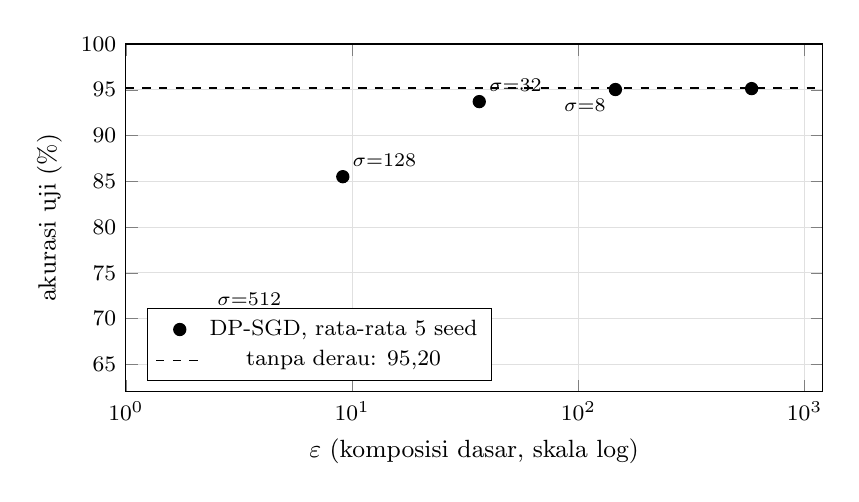
\begin{tikzpicture}
\begin{axis}[
  width=0.86\linewidth, height=6.0cm,
  xlabel={$\varepsilon$ (komposisi dasar, skala log)},
  ylabel={akurasi uji (\%)},
  xmode=log, log basis x=10,
  xmin=1, xmax=1200, ymin=62, ymax=100,
  xtick={1,10,100,1000},
  ytick={65,70,75,80,85,90,95,100},
  grid=major, grid style={black!12},
  tick label style={font=\footnotesize},
  label style={font=\small},
  legend style={font=\footnotesize, at={(0.03,0.03)}, anchor=south west},
]
\addplot[only marks, mark=*, mark size=2.2pt, black] coordinates {
  (2.3,70.39) (9.1,85.51) (36.5,93.71) (145.9,95.03) (583.7,95.13)
};
\addlegendentry{DP-SGD, rata-rata 5 seed}
\addplot[black, dashed, domain=1:1200, samples=2] {95.20};
\addlegendentry{tanpa derau: $95{,}20$}
\node[font=\scriptsize, anchor=south west] at (axis cs:2.3,70.39) {$\sigma{=}512$};
\node[font=\scriptsize, anchor=south west] at (axis cs:9.1,85.51) {$\sigma{=}128$};
\node[font=\scriptsize, anchor=south west] at (axis cs:36.5,93.71) {$\sigma{=}32$};
\node[font=\scriptsize, anchor=north east] at (axis cs:145.9,95.03) {$\sigma{=}8$};
\end{axis}
\end{tikzpicture}
\caption{Akurasi uji terhadap anggaran privasi pada percobaan Lab komputasi ($n=200$,
$d=8$, $T=200$, $\delta=10^{-5}$, lima seed). Setiap titik adalah hasil eksekusi nyata,
berpasangan dengan kolom \texttt{eps\_dsr} pada keluaran. Garis putus-putus adalah
akurasi tanpa derau. Sumbu mendatar logaritmik: menurunkan $\varepsilon$ dari $36{,}5$
ke $2{,}3$ berharga $23$ poin akurasi, sedangkan dari $583{,}7$ ke $145{,}9$ nyaris
gratis.}
\label{fig:tradeoff}
\end{figure}

\begin{figure}
\centering
\begin{tikzpicture}[scale=1.15]
\draw[->, black!60] (-1.25,0) -- (1.45,0) node[right, font=\footnotesize]
  {$\operatorname{Re}$};
\draw[->, black!60] (0,-1.1) -- (0,1.25) node[above, font=\footnotesize]
  {$\operatorname{Im}$};
\draw[black!35, dashed] (0,0) circle (0.7071);
\draw[black!55, thin] (0.7071,0) -- (0.7071,0.7071) -- (0,0.7071);
\draw[black!55, thin] (0.5,0) -- (0.5,0.5) -- (0,0.5);
\draw[->, very thick, black] (0,0) -- (0.7071,0.7071)
  node[above left, font=\footnotesize] {$a_0$};
\draw[->, very thick, black] (0,0) -- (-0.7071,0.7071);
\draw[->, thick, black!55] (0,0) -- (0.5,0.5);
\draw[->, thick, black!55] (0,0) -- (0.5,-0.5) node[below right, font=\footnotesize]
  {$a_1$};
\node[font=\scriptsize, anchor=west] at (0.75,0.16) {$\tfrac{1}{\sqrt2}=0{,}7071$};
\node[font=\scriptsize, anchor=north] at (0.5,-0.55) {$0{,}5-0{,}5i$};
\node[font=\scriptsize, anchor=south] at (0.5,0.56) {$0{,}5+0{,}5i$};
\draw[black!35] (0.09,0) arc (0:45:0.42);
\node[font=\scriptsize] at (0.30,0.16) {$45^\circ$};
\end{tikzpicture}
\caption{Amplitudo sebagai panah pada bidang kompleks. Panah tebal adalah keadaan
$H|0\rangle$ dengan $a_0=a_1=1/\sqrt2$; panah tipis adalah $HSH|0\rangle$ dengan
$S=\operatorname{diag}(1,i)$, yaitu $0{,}5+0{,}5i$ dan $0{,}5-0{,}5i$. Modulusnya tetap
$0{,}7071$, jadi peluang kedua hasil tetap $1/2$, tetapi fasenya bergeser
$45^\circ$ ke arah berlawanan. Pengukuran tidak membedakan kedua keadaan itu; gerbang
berikutnya bisa. Koordinat panah diambil dari keluaran Lab komputasi, bukan ilustrasi.}
\label{fig:fase}
\end{figure}

Gambar~\ref{fig:tradeoff} adalah bentuk kuantitatif trade-off privasi-utilitas: kurvanya
tidak linear, dan bagian termahal ada di ujung kiri, di wilayah yang paling sering dipuji
di abstrak. Gambar~\ref{fig:fase} adalah bentuk geometris kalimat ``modulus menentukan
peluang, fase menentukan interferensi''.

\begin{untukdosen}
Urutan mengajar yang saya sarankan: mulai dari Gambar~\ref{fig:tradeoff}, bukan dari
definisi. Tunjukkan bahwa kurva itu punya ujung kiri yang mahal, lalu tanya mengapa.
Siswa biasanya menebak ``karena deraunya besar'', yang benar tetapi belum cukup; yang
perlu muncul adalah bahwa anggaran privasi dijumlahkan sepanjang langkah, sehingga
mengecilkan $\varepsilon$ per langkah dibayar dua kali, pada derau dan pada jumlah
langkah.

Dua miskonsepsi yang hampir selalu muncul. Pertama, mahasiswa membaca
``$(\varepsilon,\delta)$-DP'' sebagai ``model ini aman''. Yang benar, ia janji tentang
pengaruh satu catatan pada sebaran keluaran, dan model itu masih bisa salah total. Kedua,
mahasiswa mengira fase kuantum hiasan notasi karena ``peluang hanya bergantung pada
modulus''. Contoh $HZH|0\rangle$ mematahkannya dalam tiga baris.

Aktivitas papan tulis yang berhasil di kelas kami: minta dua siswa menghitung
$HZH|0\rangle$ dan $HHH|0\rangle$ secara terpisah, lalu bandingkan. Keduanya memakai
tiga gerbang, beda hanya satu matriks di tengah, dan hasilnya $|1\rangle$ melawan
$|0\rangle$. Kelas siap lanjut bila seorang mahasiswa bisa menjelaskan mengapa
$HSH|0\rangle$ memberi peluang sama dengan $H|0\rangle$ tetapi keadaan berbeda.
\end{untukdosen}

\section{Ringkasan}

\begin{ringkasan}
\begin{itemize}
  \item Model yang dilatih pada data pribadi membocorkan informasi lewat tiga jalur:
        keanggotaan, atribut, dan rekonstruksi, dan yang ketiga bekerja dari gradien.
  \item Privasi diferensial $(\varepsilon,\delta)$ membandingkan dua sebaran keluaran
        untuk data yang berbeda pada satu orang, dengan kuantor ``untuk setiap himpunan
        keluaran''. Kuantor itu yang membuat janjinya berlaku terhadap penyerang, bukan
        hanya terhadap rata-rata.
  \item Mekanisme Laplace dengan skala $b=\Delta f/\varepsilon$ memenuhi
        $(\varepsilon,0)$; buktinya hanya membandingkan rasio dua kepadatan. Mekanisme
        Gauss memakai $\sigma\ge\sqrt{2\ln(1{,}25/\delta)}/\varepsilon$ dan memberi
        $\delta>0$.
  \item Komposisi dasar menjumlahkan $\varepsilon$; komposisi lanjut memberi suku
        $\sqrt{T}$ yang lebih baik hanya bila $\varepsilon$ per langkah kecil: pada
        $\sigma=32$ hasilnya $36{,}5$ versus $20{,}6$, sedangkan pada $\sigma=2$
        hasilnya $583{,}7$ versus $11\,302{,}8$.
  \item DP-SGD memotong gradien per contoh pada norma $C$ lalu menambah derau
        $\sigma C/B$. Akurasi turun dari $95{,}20$ persen tanpa derau menjadi $93{,}71$
        persen pada $\varepsilon=36{,}5$ dan $70{,}39$ persen pada $\varepsilon=2{,}3$.
  \item Privasi diferensial menjamin sesuatu tentang individu, bukan kebenaran model;
        ia tidak menghapus bias, dan biaya utilitasnya bisa tidak merata antar kelompok.
  \item Keadaan kuantum hidup di $\mathbb{C}^{2^{n}}$; gerbang harus uniter karena
        peluang harus kekal, dan pengukuran satu-satunya langkah tidak uniter. Keluaran
        karena itu selalu berupa sampel.
  \item Simulasi klasik butuh $2^{n}$ amplitudo: $n=50$ berarti $16$ pebibyte. Fakta itu
        membatasi peniruan, tetapi tidak membuktikan keunggulan, dan sampai sekarang
        belum ada bukti keunggulan praktis QML yang mapan.
\end{itemize}
\end{ringkasan}

\section{Latihan}
\tingkat{menengah}

\begin{latihan}
\begin{enumerate}
  \item Nilai klaim ini: ``Model kami memenuhi privasi diferensial dengan
        $\varepsilon=0{,}5$, jadi tidak ada informasi pribadi yang bisa bocor darinya.''
        Nyatakan benar, salah, atau belum cukup bukti, dan sebutkan dua hal yang harus
        benar agar klaim itu berlaku.
  \item Buktikan bahwa mekanisme Laplace dengan skala $b=\Delta f/\varepsilon$ memenuhi
        $(\varepsilon,0)$ bila sensitivitas diukur dengan norma $\ell_1$ pada keluaran
        berdimensi $d>1$. Tunjukkan di mana argumen satu dimensi perlu diganti.
  \item Buktikan komposisi paralel: bila $M_1$ bekerja pada $D_1$ dan $M_2$ pada $D_2$
        dengan $D_1\cap D_2=\varnothing$, dan masing-masing $(\varepsilon_i,\delta_i)$,
        maka keluarannya memenuhi $(\max_i\varepsilon_i,\max_i\delta_i)$.
  \item Hitung $\varepsilon$ untuk jawaban acak bila peluang menjawab jujur adalah $p$
        dan sisanya dijawab acak dengan koin seimbang. Nyatakan $\varepsilon$ sebagai
        fungsi $p$, lalu tentukan $p$ yang memberi $\varepsilon=2$.
  \item Untuk kueri hitung dengan $\varepsilon=0{,}5$ pada $n=10\,000$, hitung peluang
        galat mutlaknya melebihi $10$ orang, lalu bandingkan dengan peluang yang sama
        bila kuerinya rata-rata dengan $R=1$. Periksa kedua angka dengan simulasi.
  \item Hitung $H\,S\,H|0\rangle$ dengan $S=\operatorname{diag}(1,i)$ selangkah demi
        langkah, lalu bandingkan peluangnya dengan $H|0\rangle$. Jelaskan mengapa hasil
        ukurnya sama padahal keadaannya berbeda, dan gerbang apa yang membedakannya.
  \item Untuk keadaan Bell $|\Phi^{+}\rangle$, hitung peluang hasil $01$ bila qubit
        kedua diukur lebih dulu dan hasilnya $0$; ulangi untuk hasil $1$. Jelaskan
        mengapa kedua jawaban menunjukkan korelasi sempurna.
  \item Tunjukkan bahwa $\begin{pmatrix}1&0\\0&e^{i\varphi}\end{pmatrix}$ uniter untuk
        setiap $\varphi$, lalu jelaskan mengapa gerbang itu tidak mengubah peluang pada
        basis komputasi tetapi bisa mengubah hasil gerbang berikutnya.
  \item Hitung jumlah amplitudo dan kebutuhan memori untuk $n=40$ dan $n=60$ qubit
        dengan $16$ byte per amplitudo. Nyatakan dalam satuan yang masuk akal, lalu
        bandingkan dengan kapasitas penyimpanan yang Anda miliki.
  \item Sebuah makalah menulis: ``Sirkuit kami menyiapkan keadaan dengan $2^{60}$
        amplitudo, jadi ia mengungguli simulasi klasik untuk pembelajaran mesin.''
        Sebutkan tiga pertanyaan yang harus dijawab sebelum kalimat itu diterima, dan
        untuk setiap pertanyaan sebutkan hasil seperti apa yang akan membuat Anda
        menerimanya.
\end{enumerate}

\noindent\textbf{Petunjuk untuk tiga butir tersulit.} Butir 2: tulis rasio kepadatan
sebagai hasil kali rasio per koordinat, lalu gunakan $\sum_j|a_j-a'_j|\le\Delta f$.
Butir 3: pada setiap langkah hanya satu dari dua mekanisme yang dapat berubah. Butir 10:
apakah seluruh amplitudo dipakai, apakah keluarannya bisa diekstrak dengan jumlah
pengukuran yang tidak eksponensial, dan apakah ada pembanding klasik pada tugas dan data
yang sama.
\end{latihan}

\begin{untukpeneliti}
Tiga hal di paruh pertama sering dikutip tanpa syaratnya. Pertama, definisi
$(\varepsilon,\delta)$ di sini adalah definisi Dwork, McSherry, Nissim, dan Smith (2006)
dalam bentuk buku Dwork dan Roth; syarat $\delta\ll 1/n$ berasal dari argumen penyamaran
satu individu, bukan dari kenyamanan analisis. Kedua, batas Gauss
$\sigma\ge\sqrt{2\ln(1{,}25/\delta)}/\varepsilon$ longgar untuk $\sigma$ kecil; batas
ketatnya diberikan mekanisme Gauss analitik Balle dan Wang (2018), dan selisihnya bisa
mencapai faktor dua pada $\varepsilon<1$. Ketiga, \emph{accountant} momen Abadi dan
rekan-rekan (2016) memakai subsampling, sehingga angka $\varepsilon$ yang dilaporkan
tanpa laju subsampling dan jumlah langkah tidak bisa dibandingkan dengan angka lain.

Di paruh kedua, yang benar-benar terbukti adalah pernyataan bersyarat: pemisahan
kompleksitas untuk keluarga tugas tertentu, dan ketidakmampuan simulasi klasik untuk
keadaan umum. Yang populer tetapi tidak terbukti adalah klaim bahwa sirkuit variasional
memberi keunggulan pada data klasik. Tang (2019) dan Huang, Kueng, Preskill (2021)
membatasi klaim itu dari dua arah: struktur data bisa menghapus percepatan, dan
pemisahan yang ada bergantung pada asumsi distribusi. McClean dan rekan-rekan (2018)
menunjukkan gradien yang menghilang secara eksponensial pada sirkuit dalam, sehingga
pelatihan variasional punya hambatan yang belum terselesaikan.

Pertanyaan yang paling penting bukan ``apakah ada percepatan'', melainkan ``percepatan
seperti apa yang bertahan setelah biaya pembacaan, penyusunan keadaan, dan koreksi galat
dihitung''. Sampai ada jawaban yang diukur pada perangkat keras dengan data nyata,
setiap klaim keunggulan praktis QML sebaiknya dibaca sebagai hipotesis.
\end{untukpeneliti}

\peta{Paruh privasi mengikuti Dwork dan Roth, \emph{The Algorithmic Foundations of
Differential Privacy} (bab 2--3 dan lampiran A), Abadi dkk., \emph{Deep Learning with
Differential Privacy} (2016) untuk DP-SGD, Shokri dkk. (2017) untuk inferensi keanggotaan, Dinur dan
Nissim (2003) untuk rekonstruksi dari kueri agregat, serta Zhu, Liu, Han (2019) untuk
rekonstruksi dari gradien. Paruh kuantum mengikuti Nielsen dan Chuang,
\emph{Quantum Computation and Quantum Information} (bab 2 dan 4), Cerezo dkk. (2021, 2022) untuk batas algoritme
variasional, Tang (2019) untuk dekuantisasi, dan Huang, Kueng, Preskill (2021) untuk
pemisahan berbasis data. Prasyaratnya ada pada Bab 10 (SVD dan ortogonalitas), Bab 16
(peluang bersyarat), dan Bab 17 (variabel acak), sedangkan kaitan Fourier dan konvolusi
ada pada Bab 14 dan Bab 15.}
